\documentclass[conference, a4paper]{IEEEtran}
% \documentclass{article}
\usepackage[T1]{fontenc} %%%key to get copy and paste for the code!
\usepackage[utf8]{inputenc} %%% to support copy and paste with accents for frnehc stuff
\usepackage{times}
\usepackage[scaled=0.85]{helvet}
\usepackage{graphicx}
\usepackage{ifthen}
\usepackage{xspace}
\usepackage{alltt}
\usepackage{latexsym}
\usepackage{url}            
\usepackage{amssymb}
\usepackage{amsfonts}
\usepackage{amsmath}
\usepackage{stmaryrd}
\usepackage{enumerate}

\usepackage[pdftex,colorlinks=true,pdfstartview=FitV,linkcolor=blue,citecolor=blue,urlcolor=blue]{hyperref}
\usepackage{xspace}
\usepackage{listings}


\newboolean{showcomments}
\setboolean{showcomments}{true}
\ifthenelse{\boolean{showcomments}}
  {\newcommand{\bnote}[2]{
	\fbox{\bfseries\sffamily\scriptsize#1}
    {\sf\small$\blacktriangleright$\textit{#2}$\blacktriangleleft$}
    % \marginpar{\fbox{\bfseries\sffamily#1}}
   }
   \newcommand{\cvsversion}{\emph{\scriptsize$-$Id: macros.tex,v 1.1.1.1 2007/02/28 13:43:36 bergel Exp $-$}}
  }
  {\newcommand{\bnote}[2]{}
   \newcommand{\cvsversion}{}
  } 


\newcommand{\here}{\bnote{***}{CONTINUE HERE}}
\newcommand{\nb}[1]{\bnote{NB}{#1}}

\newcommand{\fix}[1]{\bnote{FIX}{#1}}
%%%% add your own macros 

\newcommand{\np}[1]{\bnote{Nico}{#1}}
\newcommand{\jf}[1]{\bnote{Javi}{#1}}

\graphicspath{{figures/}}
%%% 


\newcommand{\figref}[1]{Figure~\ref{fig:#1}}
\newcommand{\figlabel}[1]{\label{fig:#1}}
\newcommand{\tabref}[1]{Table~\ref{tab:#1}}
\newcommand{\layout}[1]{#1}
\newcommand{\commented}[1]{}
\newcommand{\secref}[1]{Section \ref{sec:#1}}
\newcommand{\seclabel}[1]{\label{sec:#1}}

%\newcommand{\ct}[1]{\textsf{#1}}
\newcommand{\stCode}[1]{\textsf{#1}}
\newcommand{\stMethod}[1]{\textsf{#1}}
\newcommand{\sep}{\texttt{>>}\xspace}
\newcommand{\stAssoc}{\texttt{->}\xspace}

\newcommand{\stBar}{$\mid$}
\newcommand{\stSelector}{$\gg$}
\newcommand{\ret}{\^{}}
\newcommand{\msup}{$>$}
%\newcommand{\ret}{$\uparrow$\xspace}

\newcommand{\myparagraph}[1]{\noindent\textbf{#1.}}
\newcommand{\eg}{\emph{e.g.,}\xspace}
\newcommand{\ie}{\emph{i.e.,}\xspace}
\newcommand{\etal}{\emph{et al.,}\xspace}
\newcommand{\ct}[1]{{\textsf{#1}}\xspace}
\newcommand{\cf}{\emph{cf.}\xspace}

\newenvironment{code}
    {\begin{alltt}\sffamily}
    {\end{alltt}\normalsize}

\newcommand{\defaultScale}{0.55}
\newcommand{\pic}[3]{
   \begin{figure}[h]
   \begin{center}
   \includegraphics[scale=\defaultScale]{#1}
   \caption{#2}
   \label{#3}
   \end{center}
   \end{figure}
}

\newcommand{\twocolumnpic}[3]{
   \begin{figure*}[!ht]
   \begin{center}
   \includegraphics[scale=\defaultScale]{#1}
   \caption{#2}
   \label{#3}
   \end{center}
   \end{figure*}}

\newcommand{\infe}{$<$}
\newcommand{\supe}{$\rightarrow$\xspace}
\newcommand{\di}{$\gg$\xspace}
\newcommand{\adhoc}{\textit{ad-hoc}\xspace}

\usepackage{url}            
\makeatletter
\def\url@leostyle{%
  \@ifundefined{selectfont}{\def\UrlFont{\sf}}{\def\UrlFont{\small\sffamily}}}
\makeatother
% Now actually use the newly defined style.
\urlstyle{leo}


\lstset{ %
  backgroundcolor=\color{white},   % choose the background color; you must add \usepackage{color} or \usepackage{xcolor}
  basicstyle=\footnotesize\ttfamily,        % the size of the fonts that are used for the code
  breakatwhitespace=false,         % sets if automatic breaks should only happen at whitespace
  breaklines=true,                 % sets automatic line breaking
  captionpos=b,                    % sets the caption-position to bottom
  escapeinside={\%*}{*)},          % if you want to add LaTeX within your code
  extendedchars=true,              % lets you use non-ASCII characters; for 8-bits encodings only, does not work with UTF-8
  keepspaces=true,                 % keeps spaces in text, useful for keeping indentation of code (possibly needs columns=flexible)
  numbersep=5pt,                   % how far the line-numbers are from the code
  rulecolor=\color{black},         % if not set, the frame-color may be changed on line-breaks within not-black text (e.g. comments (green here))
  showspaces=false,                % show spaces everywhere adding particular underscores; it overrides 'showstringspaces'
  showstringspaces=false,          % underline spaces within strings only
  showtabs=false,                  % show tabs within strings adding particular underscores
  stepnumber=2,                    % the step between two line-numbers. If it's 1, each line will be numbered
  tabsize=2,                       % sets default tabsize to 2 spaces
}

\lstdefinelanguage{Wollok}{
  keywords={program, console, val, object, method},
  sensitive=true,
  comment=[l]{//},
  morecomment=[s]{/*}{*/},
  morestring=[b]',
  morestring=[b]"
}


\begin{document}
\title{Wollok -- Relearning How To Teach \\ Object-Oriented Programming}

\author{\IEEEauthorblockN{
Nicolás Passerini\IEEEauthorrefmark{1}\IEEEauthorrefmark{2}\IEEEauthorrefmark{4},
Javier Fernandes\IEEEauthorrefmark{1}\IEEEauthorrefmark{2},
Pablo Tesone\IEEEauthorrefmark{3} and 
Débora Fortini\IEEEauthorrefmark{2}\IEEEauthorrefmark{4}}

\IEEEauthorblockA{\IEEEauthorrefmark{1}Universidad Nacional de Quilmes}
\IEEEauthorblockA{\IEEEauthorrefmark{2}Universidad Nacional de San Martín}
\IEEEauthorblockA{\IEEEauthorrefmark{3}Universidad Nacional del Oeste}
\IEEEauthorblockA{\IEEEauthorrefmark{4}Universidad Tecnológica Nacional - Facultad Regional Buenos Aires}}

\date{\today}
\maketitle

\begin{abstract}
Students often have difficulties in learning how to program in an object-oriented style. 
One of the causes of this problem is that object-oriented languages require the programmer to be familiarized with a big amount of non-trivial concepts. 
For several years we have been teaching introductory OOP courses using an \emph{incremental learning path}, 
which starts with a simplified OOP model consisting only of objects, messages and references. 
This learning path is supported by a customized development environment which enables the creation of programs using this \emph{simplified programming model}, 
and allows us to postpone the introduction of more abstract concepts like classes or inheritance. 

In this work we propose an enhancement to this learning path focusing on the transitions between the stages of the course. 
We also present a new educational programming language named Wollok, which allows maximizing the accuracy in the selection of concepts to present. 
Finally, Wollok is accompanied by a programming environment which has lots of tools to guide the student and to help detecting mistakes
and at the same time is in line with the most common professional practices.
\end{abstract}

\section{Introduction}
\label{sec:intro}

% Context
% (a) hay que arrancar introduciendo nuestra visión, contando por qué enseñamos objetos de determinada manera, por qué hicimos Ozono.

% La importancia de arrancar con objetos. -- No sé si arrancar con esto.
\emph{Object-oriented programming} (OOP) has become the \textit{de facto} standard programming paradigm in industrial software development.
Therefore, in the last years software engineering curricula have put more emphasis in object-oriented courses.
% Furthermore, opinion in the community is divided as if it should be the first programming model to be presented. 
% Problem
Still, students often have difficulties in learning how to program in an object-oriented style which show up both in academic and in industrial environments.

Several causes have been blamed for the difficulties in OOP learning.
First, OO courses tend to focus too much on syntax and the particular characteristics of a language, instead of focusing on OOP distinctive characteristics.
Second, many OO languages used in introductory courses do require to grasp a lot of quite abstract concepts before being able to build a first program.
Finally, poor programming environments are used, although we are at a time where an unexperienced programmer could be making great use of the guidance a good programming environment could provide. These problems are not exclusive of OO courses, they are present in all the general programming courses \cite{singh2012}.

\medskip 

% Known tracks for solutions
% here you want to show that you are not an idiot not knowing what have been around

% Primero hablar de lenguajes específicos para enseñar
There have been several proposals to address the difficulties in introductory OO courses 
by defining a specific language which provides a simplified programming model such as Karel++ \cite{bergin_karel++:_1996} and Mama \cite{harrisonmama}.
This approach has been used even outside the OO world \cite{feurzeig_programming-languages_1970, pattis_karel_1981, lopez_nombre_2012}.
% Environments
A step further is to provide a whole programming environment specifically designed to aid novice programmers 
such as Squeak \cite{ingalls_back_1997}, Traffic \cite{broy_outside-method_2003} and BlueJ \cite{bennedsen_bluej_2010}. 

% Object first
The great differences between these programming languages and environments show that they have to be analyzed in the light of the pedagogical approaches behind them.
The tools are of little use without this pedagogical view.
For example, some educational languages and environments are designed to be used in \textit{object-first} approaches, 
\ie for students without any previous programming knowledge \cite{arnow_introduction_1998, bruce_library_2001}.
% Children
Other languages are focused on teaching to children or teenagers, such as Scratch \cite{malan_scratch_2007} and Etoys \cite{lee_empowering_2011}. 
% Visualization
Finally, there are many approaches which emphasize the importance of \emph{visualization tools} 
to simplify the understanding of the underlying programming model \cite{cooper_teaching_2003, roberts_designing_1998}.

\medskip
% Nuestro trabajo

Previous works from our team \cite{lombardi_instances_2007,lombardi_carlos_alumnos_2008,griggio_programming_2011,spigariol_lucas_ensenando_2013} have described an approach consisting of
(a) a novel path to introduce OO concepts, focusing on objects, messages and polymorphism first, while delaying the introduction of classes and inheritance and 
(b) a reduced and graphical programming environment which supports the order in which we introduce the concepts, by allowing to build OO programs without the need of classes.
Our approach focuses on the concepts of object, message, reference and object polymorphism, while delaying the introduction of more abstract concepts such as types, classes and inheritance.
These way of organizing a course provides a more gentle learning curve to students and allows them to write completely working programs from the first classes.

% What our solution is \ct{Set} and \ct{OrderedCollection} (so that the reader knows where the paper is going)
% Contribution of the paper
% (b) lo que aprendimos en estos 8 años haciendo eso, que nos lleva a querer darle una vuelta más.
While this approach proved to be successful in providing the students with a more profound knowledge of OOP at the same time as raising pass rates, 
we feel that there is still room for improvement, in four areas:
(a) integrating object-based and class-based programs together,
(b) creating automatic ways to produce a graphical user interface (GUI),
(c) enhancing the programming environment with a type inference tool \cite{Miln78a} that helps avoiding some common mistakes
and (d) narrowing the distance between our language and tools with those more frequently used in industrial development.

In this paper, we describe our pedagogical approach to teaching OOP\footnote{For space reasons, this paper is focused on the differences with our previous works. 
For a more comprehensive description of the base ideas, please refer to \cite{lombardi_instances_2007,lombardi_carlos_alumnos_2008,spigariol_lucas_ensenando_2013}.}.
Also, we describe a new language named Wollok, which we built to enable putting this ideas into practice in actual courses\footnote{Wollok is open-sourced and distributed under LGPLv3 License\footnote{http://www.gnu.org/copyleft/lgpl.html}.
Source code and documentation can be found in Github (\url{https://github.com/uqbar-project/wollok}).}.

\np{No sé si hablar de los temas de colecciones, son un poco particulares de Ozono.
También del environment se podrían decir más cosas que sólo el sistema de tipos.}
\pt{Yo no hablaria de nada de eso.}

\medskip 
% Paper structure
The rest of the paper is structured as follows. In \secref{problem} we present the problems of learning Object Oriented programming, and the consequences of this difficulties to the students. \secref{wollokLanguage} describes the proposed language and the design goals and ideas we take in consideration for it. In \secref{environment} we describe the integrated development environment we have developed for Wollok and all the features it has and how they are useful for the teaching of programming skills. \secref{discussion} analyses the different design decisions we have taken, while \secref{related} compares our solution with another similar approaches. Finally, we summarize our contributions in \secref{conclusion},
along with some possible lines of further work derived from this initial ideas. As an appendix we have Sections \ref{sec:implementation}, \ref{sec:wollokSoftware} and \ref{sec:ChecksAndValidations} which give more details about the implementation.



\section{Problem Description}
\label{sec:problem}

% Context, exposed with the \textbf{most precise terms possible} (don't open unwanted doors for the reader)

% Los cursos se enfocan en sintaxis y usan lenguajes inadecuados.
One cause behind the difficulties in learning OOP is that courses often focus on syntax and the particular characteristics of a programming language, 
leading students to concentrate on these relatively unimportant details,
rather than the underlying object-oriented modelling skills. 
Also, the use of industrial languages to introduce OOP requires the student to understand several concepts before being able to run his first program. \cite{kolling_problem_1999}

% Ejemplo con Java.
By focusing on those details, many students fail to comprehend the essential model that transcends particular programming languages \cite{the_joint_task_force_on_computing_curricula_computing_2001}. 
Figure \ref{fig:helloWorld} shows a typical first program, written in Java \cite{arnold_java_1996}.
To get this program running, the student has to walk through a minefield of complex concepts: packages, classes, scoping, types, arrays and class methods among others.
However, he is still unable to do more basic OO programming, such as sending a message to an object.

\begin{figure}[ht]
 \centering
 \begin{lstlisting}[language=Java]
	package examples;
	
	public class HelloWorld {
		public static void main(String[] args) {
			System.out.println("Hello World");
		}
	}
 \end{lstlisting}
 
 \caption{\small Sample initial Java program which diverts student attention from the most important concepts.}
 \label{fig:helloWorld}
\end{figure}

% Por eso los pibes no aprenden
For all these reasons, courses tend to spend too much time concentrated on the mechanistic details of programming constructs, 
leaving too little time to become fluent on the distinctive characters of OOP, 
such as identifying objects and their knowledge \emph{relationships}, assigning \emph{responsibilities} 
and taking advantage of \emph{encapsulation} and \emph{polymorphism} to make programs more robust and extensible.

% Además necesitamos environments
To make things worse, frequently the students do not have proper tools that could help them overcoming all the obstacles.
Already in 1999, Kolling \etal had established the importance of environments in introductory courses \cite{kolling_problem_1999}. 
He stated that earlier introductory courses focused on the development of algorithms in procedural or functional languages. 
To do this, an editor and a compiler was all that was needed for the practical part of the work. 
Modern courses now use object-oriented languages and subject material taught includes testing, debugging and code reuse. 
This creates the need to deal with multiple source files and multiple program development tools from the very start. 
To give a beginning student a chance to cope with this increased complexity, better environment support is needed. 

\medskip

% Probably set the vocabulary before to cut any misinterpretation
% Problem

% Consecuencias en la acadamia y en la industria
The failure of students to understand the essential object-oriented concepts shows both in academy as in industry.
In academic environments we find very low completion rates in introductory OO courses.
Moreover, students in their very beginning of an informatics career which fail their introductory programming courses, are often likely to give up their studies \cite{milne_2002}.
In industrial development, we find that these hindrances reduce the opportunity of students to apply the concepts of the paradigm effectively in their further professional practice, 
resulting in several IT-projects not taking advantage of the possibilities offered by the potential of good object-oriented practices \cite{lombardi_instances_2007}.

\medskip 

% Factual solution tracks, to position...
\np{Contar algo de otras propuestas anteriores a la nuestra}
\pt{No se si pondria algo, ya estan en los trabajos anteriores que estan citando. Podemos decir que lean el tuyo con carlono.}

Our previous work in this area is based on the proposal to change the order of subjects in OOP introductory coures \cite{lombardi_instances_2007}, 
starting with a \emph{Simplified Programming Model} (SPM) which includes only the most basic OOP concepts, such as objects, messages, references, methods and dynamic dispatch.
The aim of the SPM is to provide students with the minimal set of concepts that allows them to write OO programs, exploiting polymorphism right from the beginning of the course.
This foundations allow for an \emph{Incremental Learning Path}, \ie more abstract concepts can be added later, 
giving the student the time to be familiarized with one concept before introducing the next one.

To enable this we provided a simplified OO language with an ad-hoc educational programming environment 
named Ozono\footnote{The name has been changing along these years. Other names for our programming environment have been ObjectBrowser, Loop and Hoope}, 
in which students can create objects and define their behavior directly, without the need for classes and inheritance \cite{griggio_programming_2011}.
Ozono is based on Smalltalk\footnote{The latest version currently in use in universities is based on a Smalltalk dialect named Pharo \cite{black_pharo_2010}.}.
and thus it is a \textit{dynamic language}.

We take special advantage of the dynamic characteristic of the language because it allows very simple uses of polymorphism, 
\ie any two objects that understand a common set of messages can be treated polymorphically without worrying about inheritance or \emph{interface} implementation,
which is indispensable if we want them to exploit polymorphism already in their programs after only two or three lectures. 

Another interesting advantage is the ability to interact with the objects directly, sending different messages to them and see how they react. 
This interactive sessions increases the understanding of the paradigm and the way the responsibilities are distributed in an object oriented program.

\medskip
This approach produced impressive results and therefore has been adopted in other courses and universities.
The simplified programming model, allows the students to spend more time working with the essential concepts of the OO paradigm.
This, in turn allows for more practice and more complex exercises, even incorporating more advanced OO techniques such as \emph{design patterns} \cite{Gamm03a},
which in traditional approaches are normally postponed to a second OOP course.

% Esto podría extender la descripción del problema
%  Ozono hereda muchos de los problemas de los entornos Smalltalk

% Smalltalk, however, lacks other important facilities: no visualisation tools for class
% relations are available. The main problem with this lies in the Smalltalk language 
% itself: since it is not statically typed, it is not possible to extract usage relations fromo
% its source code. No indication exists before runtime as to the call relationships
% between classes. Inheritance relationships as shown in the browser do not present
% the relationships of one application but rather the whole Smalltalk environment and
% so the browser is not used as an application modelling tool. .
% Reports about the use of Smalltalk systems for teaching also point to another
% problem: its size. While the language itself (in terms of the number of constructs) is
% small, the class library and tools are large and often confusing. Several authors
% reported difficulties with the students ability to cope with the environment [7, 8],
% especially that experimentation and self directed learning was not working well
% because students were overwhelmed by the system. They also found that the
% functionality of the browser should be limited, since its power and flexibility caused
% more problems than it solved. \cite{kolling_problem_1999}.


% Our solution in a nutshell.
% (c) las ideas nuevas... y wollok como herramienta para dar soporte a esas ideas.

% Our solution: approach
Still, the experience of eight years in four universities\footnote{Ozono is currently used in Universidad Tecnológica Nacional, F. R. Buenos Aires and F.R. Delta and 
Universidad Nacional de Quilmes; and it have been used in Universidad Nacional de San Martín and Universidad Nacional del Oeste.}
and thousands of students has provided us with new insights of the learning process, 
which is what lead us to introduce several adjustements in our approach.

In the first place, starting with a \emph{classless} language mandates a change of language and enviroment in the middle of the course,
which is confusing for some students. 
To solve this, we propose to integrate \emph{class-based} and \emph{standalone objects} in the same language.
\np{Ver bien qué nombres les ponemos y definir los conceptos antes.}
\pt{Me incline por standalone object, porque es lo que se usa despues.}

Second, we think that the absence of static typing information (which Ozono inherits from Smalltalk) prevents our programming environment to aid the students in finding some typical beginner mistakes.
Still, we do not want to force the students to add type annotations to their code, because that would distract them from the concepts we want to focus on.
We propose to settle this apparent controversy by enhancing our programming environment with a type inferer.
By doing so, the student is not required to care about type annotations, and at the same type we can detect some programming mistakes and aid the student in solving them.

Last, we have detected that sometimes the students which seem to understand the main concepts and can apply them in interesting ways to create medium to complex program, 
then have a hard time translating this knowledge to their professional activity.
We think that a good mitigation plan for this problem starts with bringing the activities in the course as close as possible to the professional practice.
For that matter, we propose to incorporate industrial best practices such as code repositories and unit tests, adapted to the possibilities of students with little or no programming experience.

\medskip
% Our solution: environment
The renewed approach is supported with a new programming language, named Wollok, and a programming environment which aids students to write, test and run programs.
Wollok is designed to give support to our pedagogical approach; 
it allows to define both classes and standalone objects,
incorporates a basic type inferer
and provides a simple syntax to define unit tests.

A big difference with Ozono and other educational OO languages is that Wollok is a \emph{file-based} language.
While we recognize the value of the \emph{image-based} approaches, we also are aware that most industrial programming enviroments are file-based.
Therefore, we think that a file-based approach will shorten the distance between the classroom and the professional activity, which is one of our main goals.
Moreover, image-based enviromnents tend to blur the distinction between the programming environment and the program under development,
which can embody great possibilities for advanced programmers but often does not more than confuse beginners.
Also being file-based allows the usage of the most popular code
repositories such as Git, and also reduces the gap for integrating the language with existing tools like code-reviewing, static code analysers and code coverage tools. 
This tools can be easily integrated to the programming environment, giving the student the a simplify introduction to these professional tools.

Finally, the programming enviroment incorporates several advanced characteristics from professional environments, 
which improves the coding experience, and at the same time allows the student to familiarize himself with the kind of tools he will face in his later professional activity.
For that matter, the environment incorporates content assist, automatic refactorings, advanced code navigation, 
language semantics-aware search tools and error highlighting \emph{while-you-type}

\medskip
% Contribution

It is important to notice that neither the Wollok language nor the programming environment contain novel features that are unseen in industrial tools.
Therefore, the distinctive characteristic of these tools is the search for a programming environment which 
(a) supports our pedagogical approach,
(b) feeds the student with a set of tools which are adequate to his current knowledge
and (c) gently prepares him to be using industrial-level tools constitutes a novel way of dealing with the problems of OOP teaching.

A big amount of effort in our research has been put in looking for solutions that can solve the apparent controversy between the objectives (b) and (c).
Often, the rich set of tools an industrial language or programming environment offers, cannot be exploited by an unexperienced programmer or even confuses him.
On the other end, we think that poor programming environments fail to help the students to make his first steps in programming and so trims the possibilities of introductory courses.
Therefore, there is much to gain from a language that has the exact features a teacher wants to teacher
and a programming environment which provides the exact tools a student can take advantage off at each time of his learning process.

% Constraints that influenced the solution (because the solution is not
% universal) \emph{e.g.} our requirements for a solution, possibly not all
% satisfied. They should be sound and believable. Analysis of the criteria.
% Imagine that you are another guy having this problem do the constraint
% matches yours so that you could apply the solution
The current study and development has been focused on university students which have had a previous subject on inperative programming.
The natural extension of this work is the adaptation of these ideas to teenagers or more generally students without any prior programming experience.

\section{Wollok: The Language}
\label{sec:wollokLanguage}

% Free form, variable number of sections, technical details.
% But in general do not mix solution and discussions/possible variation let that for discussion

Wollok is a brand new language, built to specifically give support to our pedagogical approach.
Many ideas have been inherited from our previous projects, such as Ozono or Loop. 
The most important of these inherited characteristics is the ability to create objects and treat them polymorphically without the need of type annotations, classes or inheritance.
Also, as its predecessors and unlike other pedagogical tools, Wollok is a \emph{general purpose} language, \ie it is not tied to any specific domain.

\medskip
One of the main objectives of building a new language is to provide a smoother transition from the first phase of the course,
in which students use a \emph{simplified programming model} (SPM) and the second phase, in which they use a full-fledged OOP language.
With our previous programming tools students were required to discard, in the middle of the course, the programming model and enviromnent they already knew and were used to.
This transition has sometimes been traumatic, because the process to define an object has to be re-learnt and the tools they had been using up to that point are no longer available.
With our new approach, the tools they first learnt are going to continue being available through all the course, together with the new ones that are incorporated in later lectures.
This is also consistent with some modern industrial OO languages that allow to define both classes or standalone objects, such as Scala \cite{Oder04a}.

\medskip
Also we reduced to a minimum the syntax and the most basic constructs of the language.
While this objective was already present in our previous work, the implementation strategy of Wollok allows us to go much further in accomplishing this goal, \cf Sec. \ref{sec:implementation}.
The example in figure \ref{fig:helloWorld/wollok} shows how the classical hello world would look in Wollok.
To build this first program students are not required to know about typing, scoping or packaging.
The only required construct is the \lstinline[language=Wollok]{program} and the only command is a message send.
Both the receiver and the parameters are built-in objects which will be handled in the same way as user-defined objects.
The concepts required to understand this program are no more than program, object, message and argument passing.

\begin{figure}[ht]
 \centering
 \begin{lstlisting}[language=Wollok]
	program {
		console.println("Hello World!")
	}
 \end{lstlisting}
 
 \caption{\small Sample initial Wollok program.}
 \label{fig:helloWorld/wollok}
\end{figure}

\medskip
% Effect
\np{Esto requeriría una mención en la intro, o en general una explicación más detallada.}
Another concept we propose to emphasize in the first programming courses is the control of side effects, 
\ie a programmer should be aware of the potential side effects of each portion of code.
The most basic feature in Wollok to control side effects is the ability to 
differentiate variables (defined using \lstinline[language=Wollok]{var})
from constants (defined using \lstinline[language=Wollok]{val}).
One step forward is to incorporate an \emph{effect system} \cite{nielson_type_1999}, \cf Sec. \ref{sec:furtherWork}.

\medskip
% Misceláneos
% Profundizar y pulir el highlighting the conceptos primarios y la estratificacion de conceptos
To sum up, there are several simple features which help structure the way a student sees his programming activity.
\emph{Object literals} and \emph{collection literals} reduce boilerplate on object creation, 
since we think that the excess of bureaucracy to create an object helps to build up 
the belief that using objects or collections is far more complicated than using numbers or strings, which in turns leads to \emph{primitive obsession} \cite{fowler_refactoring:_1999}.
% Objetos no como un elemento de la IDE -Ozono: nueva referencia global, sino como un elemnto del lenguaje. Evita referencias globales.

Each Wollok file has to be defined as \emph{program}, \emph{library} or \emph{test}.
Only programs and tests can be run. Libraries can only be \emph{imported} from programs, tests or other libraries.
This concepts push students onto modularizing their programs into smaller units that can be reutilized.

Figure \ref{fig:polymorphism} shows some of the mentioned features.
The programs includes two objects which are treated polymorphically, collections and block closures.
Students should be able to build such a program after four lectures.
In the first lecture we introduce objects, messages, methods and references;
in the second one we focus on polymorphism;
and in the following two we work with blocks and collections.

\np{Acá falta hablar de la diferencia entre objeto y referencia}

\begin{figure}[ht]
 \centering
 \begin{lstlisting}[language=Wollok]
	program myProgram {
		val optimistic = object {
			method hiThere() {
				"Hi, what an amazing day !"
			}
		}

		val pessimistic = object {
			method hiThere() {
				"Don't talk to me, it's a terrible day!"
			}
		}
		
		val all = #[optimistic, pessimistic]
		
		console.println(all.map[p| p.hiThere()])
	}
 \end{lstlisting}
 
 \caption{\small Simple polymorphism example.}
 \label{fig:polymorphism}
\end{figure}

\section{Classroom Experience with wollok}
\label{experience}

Since March 2015 Wollok is being used on the Universidad Nacional de San Martín, on a subject named Algoritmos 1, where the main purpose is to introduce OOP to students with minimal experience on structured programming.
In this sections we tell our experience using for the first time, this new language to teach OOP concepts.

%Lo simple que les resulto a los chicos trabajar con una IDE
First of all, lets describe how the introduction of the students to a new IDE was. In Wollok IDE, there are just two windows, one to code objects and classes, and the other to test the objects behavior (the Repl). The use of the first window resulted very easy for them since they are coding everything in one single place, using IDE tools just as auto completion, syntax correction and syntax coloring. For more advanced student, Wollok lets you separate the code in different files, but at first, you can have everything together so you can see all the object and the relations between them.
The syntax for the REPL is the same, with the advantge that you can see at any moment without any extra work the state of any object you defined. Just writing on the REPL window the name of the object, shows its state, without any print method defined.

%La simple migración de objetos a clases.
Writing the definition of a class is not very different from writing the definition of an object, the difference is in the concept. So, we first explain to them what an object is, we write the definition of it, we see how it works. Once the students are familiar with objects and the way in which they relate with each other, we move to show how to define objects using classes, so we can create multiple objects, with the same definition, and different state.

%Los patrones de diseño que aparecieron que son muy modernos, con el uso de objetos. Era muy simple ver que usaban objetos donde antes se usaban value objects.
Some design patterns just appeared. Modelling with design patterns is not an essential part of our subject, we just introduce them to OO paradigm. But we have seen how some design pattern just appear, resulting very natural for the students. For example, having a single object with some information that other objects need (Singleton), since Wollok named objects are globally are accessible\footnote{accessibility rules are still under discussion \cf Sec.\ref{sec:discussion}}. Also, since defining classes and objects in Wollok is very succint, it is frequent the emergence of small objects that configure quiet complex colaboration patterns such as Strategies or States\cite{Gamm93b}.



\section{A Customized Programming Environment}
\label{sec:environment}

Beginner programmers are likely to require more guidance and make more mistakes than experienced programmers.
Therefore, we think that is much to gain from a good programming environment which structures the programming experienced and helps the students to identify common mistakes.

The Wollok programming environment includes a lot of features that provide guidance to the student.
\emph{Content assist} shows the students what are his possibilities at any moment and feeds automatically into the code the most usual constructs, 
allowing the student to concentrate less on syntax and more in the modelling of the exercise problem.
\emph{Quick-fixes} allow Wollok not only to highlight problems in the student's code but also to propose automatic solutions for some usual mistakes.
\emph{Advanced code navigation} and \emph{smart reference searches} allow the programmer to better understand the dependencies in his program.
Moreover, \emph{automatic class diagrams} provide a high level view of the program and also helps understanding.

% Detect mistakes
\subsection{Detecting mistakes}
The programming environment has many tools intended to help detecting mistakes.
We make special emphasis in detecting errors \emph{while} the student is writing code. \np{Acá se podría hablar más}
\emph{Syntax highlighting} helps identify the most simple mistakes by providing immediate feedback when something is not right. 
Moreover, the environment provides \emph{real-time highlights} for several kinds of mistakes (\cf \figref{check-noMethodOnThis.png}).
Finally, the \emph{type inferer} allows to detect more subtle mistakes.

\begin{figure}[ht]
    \centering
	\includegraphics[scale=0.5]{images/wollok-paper-check-noMethodOnThis.png}
    \caption{Detection of an error on sending a message to \emph{this}}
    \label{fig:check-noMethodOnThis.png}
\end{figure}

% Este no sé cómo ponerlo, es muy crítica al smalltalk.
% 8-reducir errores frustrantes: se cancela la edicion por tener 1 solo editor de metodo por ves (poder visualizar más que un sólo método simul), evitar errores de imagenes)

This validations are organized and shown in a unified way, using a dedicated section of the user interface for their display.
All the results of the checking and the validation of the program is shown in one integrated view, it is called \emph{Problems View}, Fig. \figref{problemsview.png} shows a view of this feature. 

\begin{figure}[ht]
    \centering
	\includegraphics[scale=0.5]{images/wollok-paper-check-problemsview.png}
    \caption{Problems View: shows the different problems detected by the IDE }
    \label{fig:problemsview.png}
\end{figure}

Checks and validations are not only used to show type errors or syntax errors, 
but also to encourage some properties of the program we consider as main topics in the learning process of an OO language.
Here is a list of all the validations and checks the tool supports, and a brief reason why they are useful while teaching object oriented programming:

\begin{itemize}
  \item \textbf{Syntax Errors}: this category involves all the errors detected by the parser and the lexical analyser of the language.
  \item \textbf{Style Errors}: this category is useful to teach good practices and to start to talk about code quality, reuse and code sharing.
	\begin{itemize}
		\item \textit{Case in Names}: respecting the difference case conventions for
		names (\eg using \textit{camelCase} starting with lower case for variables,
		using camel case starting with upper case for classes).
		\item \textit{Order and grouping}: inside the definition of an object or class the internal references are declared first, then the constructors and finally the methods.
		\item \textit{Modularization}: the classes can only be defined in a library and not in the main program.		
		\item \textit{Duplicated references}: it is impossible to declare a reference using a already used name. 
			This encourages the idea of avoiding name shadowing and improves the readability of the program.
	\end{itemize}
  \item \textbf{References resolution problems}: this errors are useful to detect and avoid references to undeclared variables and also errors in the sending of messages.
  
	\begin{itemize}
	  \item \textit{Undeclared references}: from local variables, parameters or internal fields of objects and classes.
	  \item \textit{Undefined constructors}: checking for the number and type of the parameters.
	  \item \textit{Messages to this}: sending messages to this is a special case, here we can check the existence of the correct method by the number and type of the arguments, even without using type inference.
	\end{itemize}
	
  \item \textbf{Reference usage}: 
		these errors are useful for the detection of erroneous or \textit{dead code}, such as unused variables or references, 
		sending messages to never assigned variables, using variables instead of values, existence of the overridden method.
		\figref{} shows an example of an unused variable error.

  \item \textbf{Type Errors}: the errors are useful for the validation of the compatibility between the references, its possible types, and the messages sent to them, this is performed by the type system and its inferer (\eg message sending, assignation of variables).
\end{itemize}

\begin{figure}[ht]
    \centering
	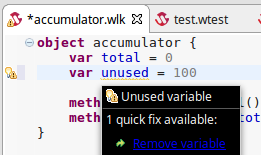
\includegraphics[scale=0.5]{images/wollok-paper-check-unusedVariable.png}
    \caption{Detection of unused variables}
    \label{fig:check-unusedVariable.png}
\end{figure}

\subsection{Type Inference}
% Type inferer
Another distinctive characteristic of the Wollok project is the type inferer.
We think that type inference is key to a simple programming environment.
On one side, it allows to detect lots of common mistakes \emph{before running the program}:
if an object does understand a message, if a wrong argument is passed, if incompatible types are mixed or even miss-spellings.
In environments without this capability it takes more time to detect errors.
Moreover, it is not uncommon that a type mistake produces a runtime error in a place different from where the mistake was done, producing confusion.

Still, providing a type inferer for a language such as Wollok has many subtleties, which deserves an independent study \cite{passerini_nicolas_extensible_2014}.
On one side we require it to be able to work without type annotations and at the same time provide feedback useful for an inexperienced programmer.
On the other side, the type system is rather complex;
for example, the presence of stand-alone objects requires the type system to handle \emph{structural types}, since a named type system would not allow them to be treated polymorphically.
Also, we want to be able to treat polymorphically stand alone objects with class-based objects.
\figref{check-messageSending.png} shows an error detected by the type inferer and how it shows the information to the programmer.
Notice that the inferred type for the object \code{ufo} is a structural type: \code{fly}

\begin{figure}[ht]
    \centering
	\includegraphics[scale=0.5]{images/wollok-paper-check-messageSending.png}
    \caption{Type system in action, detecting not defined method for the message sent}
    \label{fig:check-messageSending.png}
\end{figure}

\subsection{Beyond showing mistakes}
The IDE does is not restricted to showing what is wrong, but also generates proposals known as \emph{quick fixes}.
\figref{quickfix.png} shows an example of one of such proposals. 
In this case the IDE detects that we are sending a message that the receiver does not understand and proposes to create the corresponding method.

\begin{figure}[ht]
    \centering
	\includegraphics[scale=0.5]{images/wollok-paper-quickfix.png}
    \caption{Quick fix tool for common errors and mistakes}
    \label{fig:quickfix.png}
\end{figure}

All these tools allow the student to gain more control of his code, keeping him away from feeling lost, 
which is otherwise a common situation for a student walking his first steps into programming.
In this way the IDE becomes useful in the objective of teaching programming concepts, instead of only showing syntax errors.



\section{Discussion}
\label{sec:discussion}

% Discussion of actual solution \emph{vs.} initial constraints from \ref{sec:problem}. Explain the space of the solution, why we made it this way.
% Evaluation of the solution. How does the solution meet the criteria? Where does it succeed or fails...

A common point of controversy is whether is is worth to create a brand new language and toolset, 
instead of building our pedagogical ideas on top of existing ones, such as Self, Ruby, Smalltalk or even Eiffel.
In our experience, begginning programmers require different features from their working environment that advanced programmers
and the right selection of tools and concepts can produce substantial improvements in the learning process.
Therefore, we believe that the possibility of fine tuning provided by a specialized environment largely pays for the additional effort.
% y que muestran las grandes posibilidades que se dan a partir de esta decisión inicial: imports, tests y manejo de propiedades.

The design of Wollok import system illustrates the kind of decissions we are able to make thanks to having a specialized learning language and toolset.
By \emph{import system} we mean the way that a programming language allows the programmer to refer in one unit of code (for example a file) to program entities defined elsewhere.

\medskip
In many languages, like C or Ruby, the default behavior is that one can only refer to \emph{programming entities} (such as classes, functions, etc) defined in the same 
file\footnote{Even, in many cases, the definition must occur in the file before the usage to be legal.}
These languages usually provide the notion of an \emph{include}, 
which somehow has the effect of copying the contents of the included program file into another one.
The unstructured nature of this reuse mechanism has many drawbacks, 
because it yields a single namespace with the contents of the two or more files, 
without a clear mechanism to deal with name conflicts.
Also, file-based includes often require the programmer to be aware of the organization of the program files in directories in order to properly locate the file to be included.
Certainly we do not desire to confront beginning programmers with this kind of subleties.

Other languages, such as Java or C\# provide a more structured way to handle imports. 
In this case, a \emph{classpath} is defined, which contains all the definitions (\ie classes) in a \emph{project}.
To univocally identify classes, they are organized in \emph{packages} and each class \emph{full name} is the concatenation of the name of the package with the proper name of the class.
By using the full name of the class, it can be referenced from any file in the project.
Also, the \emph{import} directive allows the program to reference the imported class by its simple name (without package).
In this way, name clashes are avoided, at the cost of introducing a new concept: the package.

Although packages are interesting programming entities because they enable programmers to better organise larger programs, 
they are of little use for a beginner, since his programs are not yet big enough to take advantage of dividing them into packages.
Moreover, this model forces the programmer to define each class in a package\footnote{It is a bad programming practice to leave classes in the \emph{root package}.}, 
and therefore the concept of package has to be introduced right in the first lecture, 
incrementing the set of minimal concepts required for the student to grasp in order to build his first program.

\medskip

Wollok's imports try to combine both models in the most suitable way for initial programming students.
On one hand, in the first part of the course, programs fit into one single file. 
Therefore, it is simpler for students if the default scope is only one file, postponing the introduction of more advanced concepts.
With this in mind, we leave aside package definitions; each file automatically introduces a java-like package without an explicit declaration.


\bigskip
% Prototype-based inheritance
One of them is whether the learning experience should provide a way to reuse
code while still in the form of stand-alone objects without classes.
We have detected that in the early stages of the course, before introducing classes or inheritance, 
it is easy to end up in situations in which it is difficult to avoid duplicating code.
Therefore, later versions of Ozono have introduced prototype-based inheritance mechanism, 
similar to that found in Self language\cite{Ungar87self:the, Ungar91organizingprograms}. 

However, practice has shown that introducing this kind of inheritance did not smooth the transition between objects and classes. Actually it made it harder.
% In addition, prototyping is an excellent abstract model for pure object languages, keeping it simple and incredible powerful.
% But there are almost no popular or industrial languages implementing it (besides Javascript which is not exactly as standard Self prototyping). 
Therefore, we decided to cut off any code-reuse mechanism for stand-alone objects.
In this scenario, the first batteries of exercises have to be carefully selected, 
in order to avoid confronting students with problems will not be able to solve gracefully.
% When duplicated code appears as part of the course, it's important to highlight that to students, and delay solving code duplication later with classes. 
% This subject will be analysed later when we can have results of the application of this approach instead of the one of Ozono.

\medskip 
% Visual tools
\np{Creo que este párrafo no debería ir en discussion}
Another interesting point of discussion is the way to integrate a visual tools to improve the understanding of the program. 
There are many different solutions to this problem. 
One approach used by several tools, like BlueJ \cite{bennedsen_bluej_2010} involves strict UML as a diagram format for showing the information.
We think that this decision is not the best option, because UML includes a lot of information which not always is relevant for an inexperienced programmer. 
We are exploring the idea to have custom diagram formats only showing information that is relevant to the teaching process. 
Furthermore, we are analysing the possibility of adding more attractive diagrams, like board games, or adding custom images and animations to objects.
Allowing the creation of basic board games, and presenting the information in a more attractive way. 
This idea is explored in Gobstones \cite{lopez_nombre_2012} but with a fixed board.

\medskip
Regarding the language grammar and syntax we have at least two points that need to be discussed. 
% Special syntax for property access
One is whether Wollok should introduce alternative
advanced syntax for several constructions like property access, or message
sending. The objective of this alternative syntax would be to reduce the amount
of code and syntax elements (\eg parenthesis, dot for sending messages, or calling getters and
setters). Modern languages such as Scala\cite{Oder04a} and
XTend \footnote{http://www.eclipse.org/xtend/} provide such syntactic sugar.
However, we need to be careful because this shouldn't confuse novice programmers.

% Type annotations
The second point regarding syntax (and actually the whole language) is whether
the language should support some kind of type-level programming. Starting from
type annotations (to fix types for example for parameters, or variables), but
also type aliases, which could come handy given the fact that Wollok has
structural-types. This of course would be an advance topic for the course.
Probably the last topic. Again this concern shouldn't confuse the student all
over the course until reached the point where types are introduced.

\np{Si hacemos una versión larga tenemos que extender esto.}
% Syntax based
Finally, an important design issue addressed by Wollok is the use of text files instead of image
based as a way of storing the programs. This decision was taken with the objective of ease the 
process of switching to an industrial language, as most of them use this way. 
This also allows the use of industrial tools like Version Control Systems, collaborative tools 
and code revisions.



\input{relatedWorks}
\section{Conclusion}
\label{sec:conclusion}

% In this paper, we looked at problem P with this context and these
% constraints. We proposed solution S. It has such good points and such not so
% good ones. 

Wollok is an educative, object-oriented programming language which is accompanied by an advanced programming environment.
Both tools are highly customized to give support to an introductory OOP course.
Our approach consists of the combination of these three cornerstones: incremental learning path, customized language and specialized programming environment.

First, we defined an \emph{incremental\np{Revisar la idea de Javi} learning path} choosing exactly which are the concepts we want to teach and the order we want to teach them.
The learning path starts with a \emph{simplified programming model} (SPM), \ie one which uses less concepts than a full-fledged OOP language.
The SPM allows the student to build simple programs without requiring more advanced concepts.
The path should attach the SPM with a good set of programming exercises, specifically oriented to be easy to build in the selected SPM.
Once the student has mastered the concepts on the SPM, we can go a step further and introduce the next set of concepts.
\np{Acá se podría hablar de constructivismo.}

Next, defining our own programming language, allows us to give full support to the selected learning path, 
avoiding the need of explaining complex concepts too soon in the course or forcing the student to write \emph{boilerplate code} which he cannot yet understand.
Finally, a good programming environment, helps detecting errors, provides guidance and most significantly allows the student to \emph{explore}.
We have found that often students are afraid to search for solutions not seen in the class or test their own ideas, 
which leads them to restricting themselves into a smaller set of concepts and tools they feel more secure about.
A controlled environment empowers students to look around and explore new possibilities.

\medskip

% Now we could do this or that.
\label{sec:furtherWork}
One major objective in our future work is the integration of more \emph{automatic user interaction} tools into the Wollok environment.
Our objective is to enable the students to have visual and interactive programs without requiring them to learn the subleties of GUI building, 
extending the ideas in Gobstones \cite{lopez_nombre_2012} to object-oriented domains.
Some advances in this area can be seen in our previous work named Hoope \cite{estefania_miguel_hoope_2013}.

The second major objective is to continue improving the detection of programming errors.
A cornerstone to achieve this goal is the type inferer, which is our current focus.
The other half of our future work in this area is a powerfull \emph{effect system} \cite{nielson_type_1999}.

Another characteristic of programming in the real world is the need to work in teams. 
The success of object-oriented languages is partly due to their advantages in group projects. 
It is necessary teach our students about the techniques needed for teamwork, right from the beginning. 
To do this, it is essential that the environment has some form of support for group work \cite{kolling_problem_1999}.
Therefore, we plan to create simplified tools to integrate wollok te \emph{version control systems}.

Also we are working in adding more automatic refactor tools, and a better type inference implementation. 
Even working on adding an effect system to detect correct usage of the language and the code conventions.

One of the important development steps to be done is the implementation of a web version or a lighter version, using less hardware requirements, 
with the aim to run the solution in small netbooks like the ones in the \emph{Conectar-Igualdad} program\footnote{http://www.conectarigualdad.gob.ar/}.

Finally, in the educational use of the tool, we will be testing it in different educational environments to get feedback about the learning experience; 
generating learning material (\eg examples, exercises, guides). As the focus of the tool is to provide a new way of teaching programming skills. 
For this objective, we will be working in collaboration with Universities, Teachers and non profit organizations.


\section*{Acknowledgements}
We want to thank all the people who participated in the ObjectBrowser, Loop, Hoope and Ozono projects, 
as well as the teachers and students that provided feedback from their use of those tools, leading us to the ideas presented here.
% This work was supported by Ministry of Higher Education and Research, Nord-Pas de Calais Regional Council, FEDER through the 'Contrat de
% Projets Etat Region (CPER) 2007-2013',  the Cutter ANR project, ANR-10-BLAN-0219 and the MEALS Marie Curie Actions program FP7-PEOPLE-2011-
% IRSES MEALS (no. 295261). 

{
\small
\bibliographystyle{abbrv}
\bibliography{wollok,Teaching,scg}
}

\section{Examples of Checks and validations}
\seclabel{ChecksAndValidations}

All the results of the checking and the validation of the program is shown in one integrated view, it is called \emph{Problems}. The figure \figref{problemsview.png} shows a view of this feature. 
There are different types of problems, because these checks and validations are not only used to show type errors or syntax errors, but also to encourage some properties of the program we consider as main topics in the learning process of an OO language.

Here is a list of all the validations and checks the tool supports, and a
brief reason why they are useful while teaching object oriented programming.

\begin{itemize}
  \item \textbf{Syntax Errors}: this category involves all the errors detected
  by the parser and the lexical analyser of the language.
  \item \textbf{Style Errors}: this category is useful to teach good practices and to start to talk about code quality, reuse and code sharing.
	\begin{itemize}
		\item \textit{Case in Names}: respecting the difference case conventions for
		names (\eg using \textit{camelCase} starting with lower case for variables,
		using camel case starting with upper case for classes).
		\item \textit{Order and grouping}: inside the definition of an object or class the internal references are declared first, then the constructors and finally the methods.
		\item \textit{Modularization}: the classes can only be defined in a library and not in the main program.		
		\item \textit{Duplicated references}: it is impossible to declare a reference
		using a name already used. This encourage the idea of not having shadowing and
		improves the readability of the program.
	\end{itemize}
  \item \textbf{References resolution problems}: this errors are useful to detect and avoid references to undeclared variables and also errors in the sending of messages.
  
	\begin{itemize}
	  \item \textit{Undeclared references}: from local variables, parameters or internal fields of objects and classes.
	  \item \textit{Undefined constructors}: checking for the number and type of the parameters.
	  \item \textit{Messages to this}: sending messages to this is a special case, here we can check the existence of the correct method by the number and type of the arguments, even without using type inference.
	\end{itemize}
	
  \item \textbf{Reference usage}: these errors are useful for the detection of
  erroneous or \textit{dead code} (\eg unused variables or references, sending
  messages to never assigned variables, using variables instead of values, existence of the overridden method.

  \item \textbf{Type Errors}: the errors are useful for the validation of the compatibility between the references, its possible types, and the messages sent to them, this is performed by the type system and its inferer (\eg message sending, assignation of variables).
\end{itemize}




\end{document}
